\documentclass[letterpaper,twoside,12pt]{article}\usepackage[]{graphicx}\usepackage[]{color}
%% maxwidth is the original width if it is less than linewidth
%% otherwise use linewidth (to make sure the graphics do not exceed the margin)
\makeatletter
\def\maxwidth{ %
  \ifdim\Gin@nat@width>\linewidth
    \linewidth
  \else
    \Gin@nat@width
  \fi
}
\makeatother

\definecolor{fgcolor}{rgb}{0.345, 0.345, 0.345}
\newcommand{\hlnum}[1]{\textcolor[rgb]{0.686,0.059,0.569}{#1}}%
\newcommand{\hlstr}[1]{\textcolor[rgb]{0.192,0.494,0.8}{#1}}%
\newcommand{\hlcom}[1]{\textcolor[rgb]{0.678,0.584,0.686}{\textit{#1}}}%
\newcommand{\hlopt}[1]{\textcolor[rgb]{0,0,0}{#1}}%
\newcommand{\hlstd}[1]{\textcolor[rgb]{0.345,0.345,0.345}{#1}}%
\newcommand{\hlkwa}[1]{\textcolor[rgb]{0.161,0.373,0.58}{\textbf{#1}}}%
\newcommand{\hlkwb}[1]{\textcolor[rgb]{0.69,0.353,0.396}{#1}}%
\newcommand{\hlkwc}[1]{\textcolor[rgb]{0.333,0.667,0.333}{#1}}%
\newcommand{\hlkwd}[1]{\textcolor[rgb]{0.737,0.353,0.396}{\textbf{#1}}}%

\usepackage{framed}
\makeatletter
\newenvironment{kframe}{%
 \def\at@end@of@kframe{}%
 \ifinner\ifhmode%
  \def\at@end@of@kframe{\end{minipage}}%
  \begin{minipage}{\columnwidth}%
 \fi\fi%
 \def\FrameCommand##1{\hskip\@totalleftmargin \hskip-\fboxsep
 \colorbox{shadecolor}{##1}\hskip-\fboxsep
     % There is no \\@totalrightmargin, so:
     \hskip-\linewidth \hskip-\@totalleftmargin \hskip\columnwidth}%
 \MakeFramed {\advance\hsize-\width
   \@totalleftmargin\z@ \linewidth\hsize
   \@setminipage}}%
 {\par\unskip\endMakeFramed%
 \at@end@of@kframe}
\makeatother

\definecolor{shadecolor}{rgb}{.97, .97, .97}
\definecolor{messagecolor}{rgb}{0, 0, 0}
\definecolor{warningcolor}{rgb}{1, 0, 1}
\definecolor{errorcolor}{rgb}{1, 0, 0}
\newenvironment{knitrout}{}{} % an empty environment to be redefined in TeX

\usepackage{alltt}
%\documentclass[sts]{imsart}
\usepackage[USenglish]{babel} 
\usepackage[T1]{fontenc}
\usepackage{lmodern} 
\usepackage[top=1.5in, bottom=1.5in, left=1in, right=1in]{geometry}
\usepackage{amsmath}
\usepackage{graphicx}
\usepackage{epstopdf}
\usepackage{enumerate}
\usepackage{amsmath}
\usepackage{setspace}
\usepackage{arydshln}
\usepackage{caption}
\usepackage{subcaption}
\usepackage[bitstream-charter]{mathdesign}
\usepackage{setspace}
\usepackage[round]{natbib}
\usepackage{soul}
\setlength{\belowcaptionskip}{12pt}
\usepackage{framed}
\usepackage{rotating}
\usepackage{hyperref}
\usepackage[hang,flushmargin]{footmisc} 
\usepackage{framed}
\usepackage{arydshln}
\usepackage{endnotes}
\usepackage{arydshln}
\usepackage{comment}
\usepackage{url}
\usepackage{lipsum}
\usepackage{pdflscape}
\usepackage{longtable}
\usepackage[capposition=top]{floatrow}
\usepackage{subcaption}
 \raggedbottom
\providecommand{\keywords}[1]{\textbf{Keywords:} #1}

\usepackage[latin1]{inputenc}
\doublespace

\newcommand*{\SuperScriptSameStyle}[1]{%
  \ensuremath{%
    \mathchoice
      {{}^{\displaystyle #1}}%
      {{}^{\textstyle #1}}%
      {{}^{\scriptstyle #1}}%
      {{}^{\scriptscriptstyle #1}}%
  }%
}


\newcommand\blfootnote[1]{%
  \begingroup
  \renewcommand\thefootnote{}\footnote{#1}%
  \addtocounter{footnote}{-1}%
  \endgroup
}

\newcommand*{\oneS}{\SuperScriptSameStyle{*}}
\newcommand*{\twoS}{\SuperScriptSameStyle{**}}
\newcommand*{\threeS}{\SuperScriptSameStyle{*{*}*}}

\newcommand{\eeq}{\end{equation}}
\newcommand{\vs}{\vspace{5mm}}
\newcommand{\vsmore}{\vspace{15mm}}
\newcommand{\letters}{\begin{enumerate}[a.]}
\renewcommand{\i}{\item}
\renewcommand{\u}{\underline}
\renewcommand{\footnotelayout}{\doublespacing}
\renewcommand{\baselinestretch}{2}
\renewcommand{\footnotesize}{\normalsize
\setlength{\footnotesep}{\baselineskip}} 
\newenvironment{nscenter}
 {\parskip=0pt\par\nopagebreak\centering}
 {\par\noindent\ignorespacesafterend}
% \let\footnote=\endnote

%--------------------------------------------------------
\IfFileExists{upquote.sty}{\usepackage{upquote}}{}
\begin{document}
\title{Graphical Presentation of Regression Discontinuity Results\blfootnote{Authors' note: We are grateful for helpful advice received from Thad Dunning and Allan Dafoe.}}
\date{}
\author{Nat\'{a}lia S. Bueno \vspace{-6mm}\\ Yale University \\ Guadalupe Tu\~n\'on \vspace{-6mm} \\ University of California, Berkeley}


\maketitle
  
During the last decade, an increasing number of political scientists have turned to regression-discontinuity (RD) designs to estimate causal effects.  Although the growth of RD designs has stimulated a wide discussion about RD assumptions and estimation strategies, there is no single shared approach to guide empirical applications. One of the major issues in RD designs involves selection of the ``window'' or ``bandwidth'' -- the values of the running variable that define the set of units included in the RD study group.\footnote{Formally, the window is an interval on the running variable, $W_0=[\underline{r},\overline{r}]$, containing the cutoff value $r_0$. The analysis then focuses on all observations with $R_i$ within this interval. Scholars have developed numerous tools to determine the right window for a given application and estimator \citep{imbens2008regression,imbens2011optimal,calonico2015robust}.}

This choice is key for RD designs, as results are often sensitive to bandwidth size. Indeed, even those who propose particular methods to choose a given window agree that ``irrespective of the manner in which the bandwidth is chosen, one should always investigate the sensitivity of the inferences to this choice. [...] [I]f the results are critically dependent on a particular bandwidth choice, they are clearly less credible than if they are robust to such variation in bandwidths.'' \citep[p.~633]{imbens2008regression} Moreover, the existence of multiple methods to justify a given choice opens the door to ``fishing'' -- the intentional or unintentional selection of models that yield positive findings \citep{Humphreys01012013}. 

In this note, we propose a simple graphical way of reporting RD results that shows the sensitivity of estimates to a wide range of possible bandwidths.\footnote{This choice is posterior to defining the estimand and choosing an estimator for the causal effect of treatment. While the plots we propose focus on presenting the sensitivity of results to bandwidth choice, we also show how they can be used to explore the sensitivity of results to these other choices. For discussions of estimands in RD design see \citet{dunning2012natural} and \citet{calonico2015robust}.} By forcing researchers to present results for an extensive set of possible choices, the use of these plots reduces the opportunities for fishing, complementing existing good practices in the way in which RD results are presented. Some empirical applications of RD designs have presented their results using plots that are in some ways similar to the ones we propose. However, this note explores the virtues of the plots more systematically (e.g., in connection with balance tests and the discussion of the RD estimator) and provides code so that scholars can adapt them to their own applications. The following paragraphs describe how RD results are usually reported in two top political science journals and the ways in which the graphs we propose can improve on current practices. An R function to construct these plots for a wide set of applications is publicly available on the \href{https://github.com/nataliabueno/Graphical-Presentation-of-Regression-Discontinuity-Results}{online Appendix}.

\section*{Reporting RD Analyses: Current Practice}

How do political scientists report the results of regression-discontinuity designs? We reviewed all papers using RDDs published in the \emph{American Political Science Review} and \emph{American Journal of Political Science}.  We surveyed these papers and coded (1) their choice of estimators, (2) whether they present any type of balance test and, (3) if they do, the window(s) chosen for this.

Out of a total of twelve RD papers published in these journals, five report results using a single estimator.\footnote{Polynomial regression is the most popular model: nine papers use a type of polynomial regression, five employ a local linear regression, and three use a difference of means (via OLS). Only one presents results using all three estimators.} Four articles present results for a single window -- usually the full sample. The remaining papers present results using multiple windows, but the number and selection of windows are neither systematic nor extensive.\footnote{\citet{gerber2011mayors}, \citet{ferwerda2014devolution} and \citet{eggers2015} are exceptions---they show the robustness of the main result using plots similar to the one we suggest here.} Seven papers present some type of balance test, but while researchers often report their main results using a handful of windows, they do not report balance tests for different windows to the same extent.\footnote{All of the papers that use local linear regressions also use a type of standard procedure to choose the ``optimal'' bandwidth -- either \citet{imbens2008regression} or \citet{imbens2011optimal}.}

\section*{A Graphical Alternative: An Example}

We use electoral data from the U.S.\ House of Representatives from 1942 to 2008 collected by \citet{caughey2011elections} and a regression discontinuity design examining incumbency advantage to illustrate how a researcher can use plots to present RD results in a transparent and systematic way. This application has two advantages for illustrating the use of these plots. First, close-race electoral regression-discontinuity designs are one of the main applications of this type of design in political science -- we are thus presenting the plot in one of the most used RDD setups, although researchers can use this type of graph in all sorts of RD designs. Second, the use of close-race RDDs to measure the effect of incumbency advantage has sparked a vigorous debate about the assumptions and validity of these designs in particular settings. Using this application allows us to show an additional advantage of the plots we propose: tests of balance and other types of placebo tests.

Figure 1 plots the estimates of local average treatment effects as a function of the running variable, here vote margin. For example, the first solid back circle represents the average difference in vote share between an incumbent party that won by 0.45\% or less and an incumbent party that lost by 0.45\% or less is about 11 percentage points. It also reports the average difference in vote share between incumbent parties that won and lost by sequential increases of 0.2\% in vote margin between 0.45\% to 9.85\%. Figure 1 has an additional feature: the solid gray line represents the results using an additional estimator that enables us to compare the effects estimated from two different estimators, across different windows, in the same plot. In this case, we present the estimated effects of party incumbency on vote share using a local linear regression with a triangular kernel, across different bandwidths. Researchers could use different estimators, such as a polynomial regression model.\footnote{We present an example of this plot using an fourth-degree polynomial regression in Figure A.1 available at the online Appendix.} Note, however, that the black circles and the solid gray line represent different quantities. The black circles represent estimates of the average causal effect for the RD study group $N$. The difference of means estimator ($Y^T - Y^C$) -- the difference between average vote share for an incumbent party minus the average vote share for a non-incumbent party -- is unbiased for the average causal effect ($\tau_{ACE}$), represented in equation (1).\footnote{See \citet{dunning2012natural} and \citet{buenodunningtunon2014} for a discussion and proofs.} The gray line presents estimates of the average causal effect precisely at the point of discontinuity ($c$). We fit a local linear regression with a triangular kernel, within the RDD bandwith, to estimate this limit parameter ($\tau_{lim}$), represented in equation (2).\footnote{We use the terms ``window'' and ``bandwidth'' interchangeably, since both denote the values of the running variable ($r$) that define the set of units included in the RD study group. However, in local linear regression with kernel smoothers, bandwidth refers to the width of the kernel.}

\begin{equation}\label{local_parameter}
\tau_{ACE} = \frac{1}{N}\sum_{i=1}^{N} [Y_{i}(1)-Y_{i}(0)].
\end{equation}

\begin{equation}\label{limit_parameter}
\tau_{lim} =  \lim_{r \Downarrow c}  [\overline{Y}_i(1)|R_i=r] - \lim_{r \Uparrow c} [\overline{Y}_i(0)|R_i=r]
  \end{equation}

The key part of the plotting function is the section that produces the estimate for each window. For this, we first pre-specify functions for each estimator. For example, for the difference of means we have:\footnote{Note that we compute the difference of means by regressing the outcome variable on a dummy for treatment assignment, with robust standard errors allowing for unequal variances, which is algebraically equivalent to the \textit{t-test} with unequal variances.}

\singlespace
\begin{knitrout}
\definecolor{shadecolor}{rgb}{0.969, 0.969, 0.969}\color{fgcolor}\begin{kframe}
\begin{alltt}
\hlcom{#Difference of mean (using OLS with robust standard errors)}
\hlstd{dom} \hlkwb{<-} \hlkwa{function}\hlstd{(}\hlkwc{rescaled}\hlstd{,} \hlkwc{treat}\hlstd{,} \hlkwc{outcome}\hlstd{)\{}
  \hlstd{model} \hlkwb{<-} \hlkwd{lm}\hlstd{(outcome}\hlopt{~}\hlstd{treat)}
  \hlstd{est} \hlkwb{<-} \hlnum{NA}
  \hlstd{est[}\hlnum{1}\hlstd{]} \hlkwb{<-} \hlstd{model}\hlopt{$}\hlstd{coefficients[}\hlnum{2}\hlstd{]}
  \hlstd{est[}\hlnum{2}\hlstd{]} \hlkwb{<-} \hlkwd{sqrt}\hlstd{(}\hlkwd{diag}\hlstd{(}\hlkwd{vcovHC}\hlstd{(model,}\hlkwc{type}\hlstd{=}\hlstr{"HC3"}\hlstd{))[}\hlnum{2}\hlstd{])}
  \hlkwd{return}\hlstd{(est)}
\hlstd{\}}
\end{alltt}
\end{kframe}
\end{knitrout}

\doublespace

We then include a loop which takes a window value and subsets the data to keep only the observations within that window. 

\singlespace
\begin{knitrout}
\definecolor{shadecolor}{rgb}{0.969, 0.969, 0.969}\color{fgcolor}\begin{kframe}
\begin{alltt}
    ests <- \hlkwd{matrix}(NA,\hlkwd{length}(windows),3) \hlcom{#object to store loop output}
    \hlkwd{for} (i in 1:\hlkwd{length}(windows))\{
\hlcom{        # select data}
        temp <- \hlkwd{as.data.frame}(data[abs_running<=windows[i],])
\end{alltt}
\end{kframe}
\end{knitrout}
\doublespace

We take this subset of the data to calculate the estimates of interest for that window, here the difference of means. The plot requires that we calculate both the point estimates and the confidence intervals. In these figures, confidence intervals are calculated using a normal approximation and unequal variances are assumed for standard errors in the treatment and control groups. If the researcher wanted to include an additional estimator, the calculation of the estimate for a particular window would also be included in the loop.\footnote{Our plot, and the accompanying documented R code, is flexible to incorporating different ways of estimating standard errors and constructing confidence intervals. For a detailed discussion of standard errors and confidence intervals in RD designs, see \citet{calonico2015robust}.} 

\singlespace
\begin{knitrout}
\definecolor{shadecolor}{rgb}{0.969, 0.969, 0.969}\color{fgcolor}\begin{kframe}
\begin{alltt}
    \hlstd{ests[i,}\hlnum{1}\hlopt{:}\hlnum{2}\hlstd{]} \hlkwb{<-} \hlkwd{with}\hlstd{(temp,} \hlkwd{dom}\hlstd{(}\hlkwc{rescaled}\hlstd{=rescaled,} \hlkwc{treat}\hlstd{=treat,}
                                  \hlkwc{outcome}\hlstd{=outcome))}

    \hlkwa{if} \hlstd{(ci}\hlopt{==}\hlstr{"95%"}\hlstd{) CI} \hlkwb{<-} \hlkwd{cbind}\hlstd{(ests[,}\hlnum{1}\hlstd{]}\hlopt{+}\hlnum{1.96}\hlopt{*}\hlstd{ests[,}\hlnum{2}\hlstd{],ests[,}\hlnum{1}\hlstd{]}\hlopt{-}\hlnum{1.96}\hlopt{*}\hlstd{ests[,}\hlnum{2}\hlstd{])}
    \hlkwa{if} \hlstd{(ci}\hlopt{==}\hlstr{"90%"}\hlstd{) CI} \hlkwb{<-} \hlkwd{cbind}\hlstd{(ests[,}\hlnum{1}\hlstd{]}\hlopt{+}\hlnum{1.64}\hlopt{*}\hlstd{ests[,}\hlnum{2}\hlstd{],ests[,}\hlnum{1}\hlstd{]}\hlopt{-}\hlnum{1.64}\hlopt{*}\hlstd{ests[,}\hlnum{2}\hlstd{])}
\end{alltt}
\end{kframe}
\end{knitrout}
\doublespace

As expected, the confidence intervals in figure 1 become increasingly smaller for results associated with larger vote margins because the number of observations is larger. This increase in the number of observations associated with larger windows can also be reported in the plot, which we do in the upper axis of figure 1. To include the number of observations as a function of window size, we order the observed values of the outcome of interest according to their value for the runing variable and allow the user to set the different number of observations that she would want to show in the plot. We calculate the number of observations at the specified values of the running variable -- then, we add the number of observations to an upper axis in the plot.

\singlespace
\begin{knitrout}
\definecolor{shadecolor}{rgb}{0.969, 0.969, 0.969}\color{fgcolor}\begin{kframe}
\begin{alltt}
  \hlcom{# as an argument in the function, the user defines nr_obs_lab, }
  \hlcom{# the labels for the number of observations she would like to include }
  \hlcom{# in the plot}

  \hlcom{# ordering the vata by the values for the running variable}
  \hlstd{data} \hlkwb{<-} \hlkwd{as.data.frame}\hlstd{(data[}\hlkwd{order}\hlstd{(abs_running),])}

  \hlkwa{if} \hlstd{(nr_obs}\hlopt{==}\hlstd{T) \{}
    \hlcom{# binding the labels with the corresponding value for the running variable}
    \hlstd{nr_obs_lab} \hlkwb{<-} \hlkwd{cbind}\hlstd{(nr_obs_lab, data}\hlopt{$}\hlstd{abs_running[nr_obs_lab])}
  \hlstd{\}}


   \hlcom{# Finally, we include an additional axis in the plot}
   \hlkwd{axis}\hlstd{(}\hlnum{3}\hlstd{,} \hlkwc{at}\hlstd{=}\hlkwd{c}\hlstd{(nr_obs_lab[,}\hlnum{2}\hlstd{]),} \hlkwc{labels}\hlstd{=}\hlkwd{c}\hlstd{(nr_obs_lab[,}\hlnum{1}\hlstd{]),} \hlkwc{cex}\hlstd{=}\hlnum{.6}\hlstd{,} \hlkwc{col}\hlstd{=}\hlstr{"grey50"}\hlstd{,}
           \hlkwc{lwd} \hlstd{=} \hlnum{0.5}\hlstd{,} \hlkwc{padj}\hlstd{=}\hlnum{1}\hlstd{,} \hlkwc{line}\hlstd{=}\hlnum{1}\hlstd{,} \hlkwc{cex.axis}\hlstd{=}\hlnum{.7}\hlstd{,} \hlkwc{col.axis}\hlstd{=}\hlstr{"grey50"}\hlstd{)}
   \hlkwd{mtext}\hlstd{(}\hlstr{"Number of observations"}\hlstd{,} \hlkwc{side}\hlstd{=}\hlnum{3}\hlstd{,} \hlkwc{col}\hlstd{=}\hlstr{"grey50"}\hlstd{,} \hlkwc{cex}\hlstd{=}\hlnum{.7}\hlstd{,} \hlkwc{adj}\hlstd{=}\hlnum{0}\hlstd{)}
\end{alltt}
\end{kframe}
\end{knitrout}
\doublespace

% \begin{figure}
%   \caption{Mean vote share difference between winners and losers by Democratic margin of victory, from 1942 to 2008}\label{fig:main_est}
% \vspace{-1mm}
%   \centerline{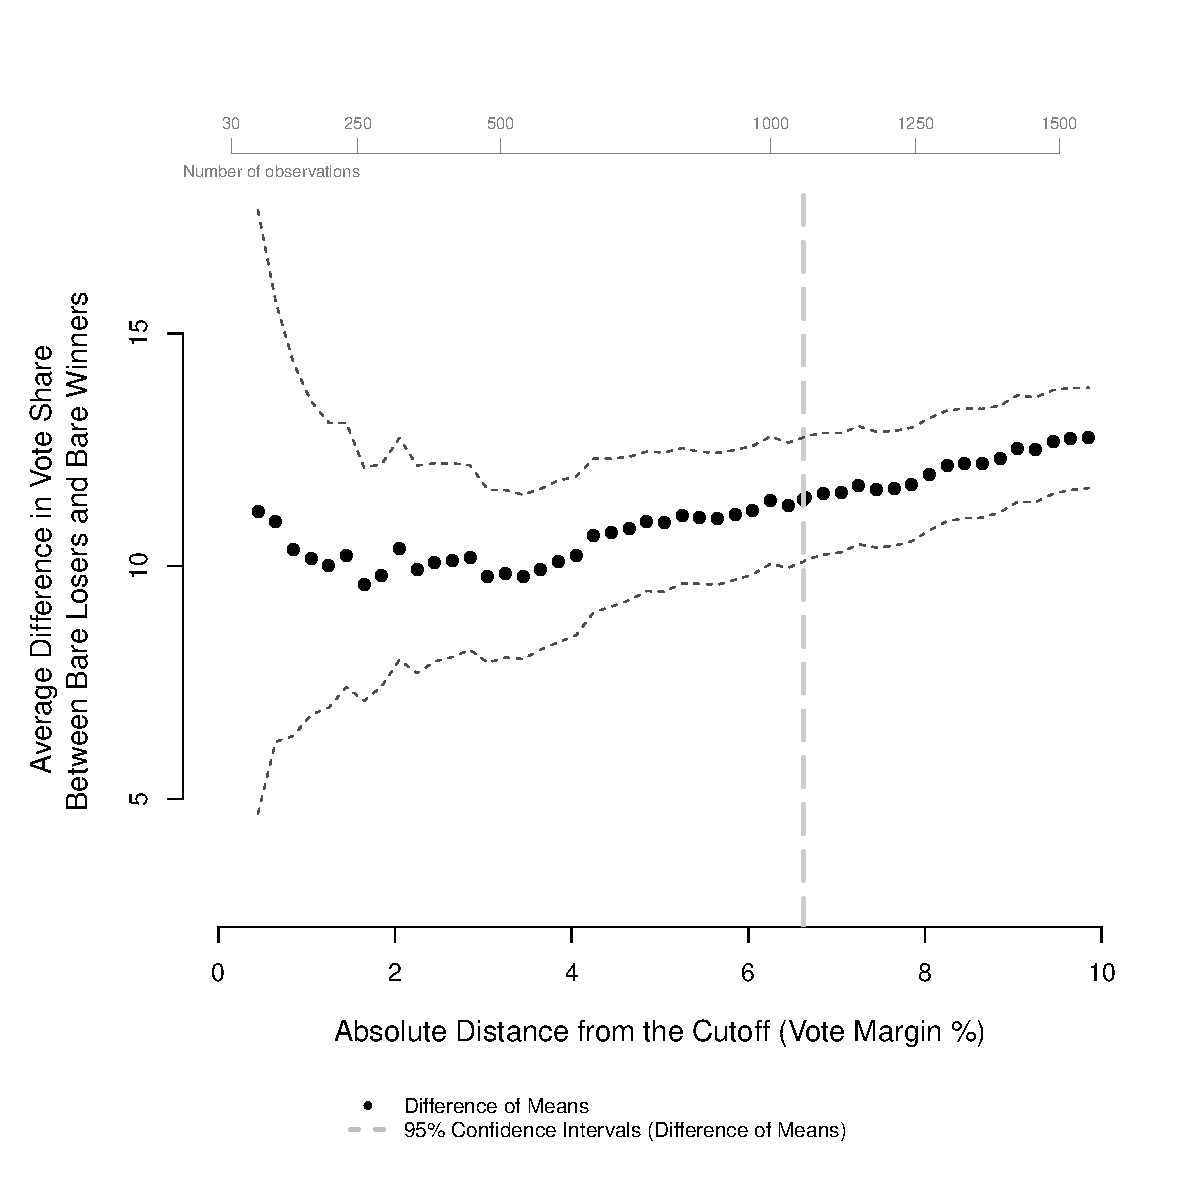
\includegraphics[width=1\textwidth]{no_add_est_plot.pdf}}
%   \floatfoot{Note: Dashed gray line at the optimal bandwidth estimated by the method of \citet{imbens2011optimal}.}
%   \end{figure}
% \clearpage

\clearpage
\begin{figure}
  \caption{Mean vote share difference between winners and losers by Democratic margin of victory in previous election, U.S.\ House of Representatives from 1942 to 2008.}\label{fig:main_est_add}
\vspace{-1mm}
  \centerline{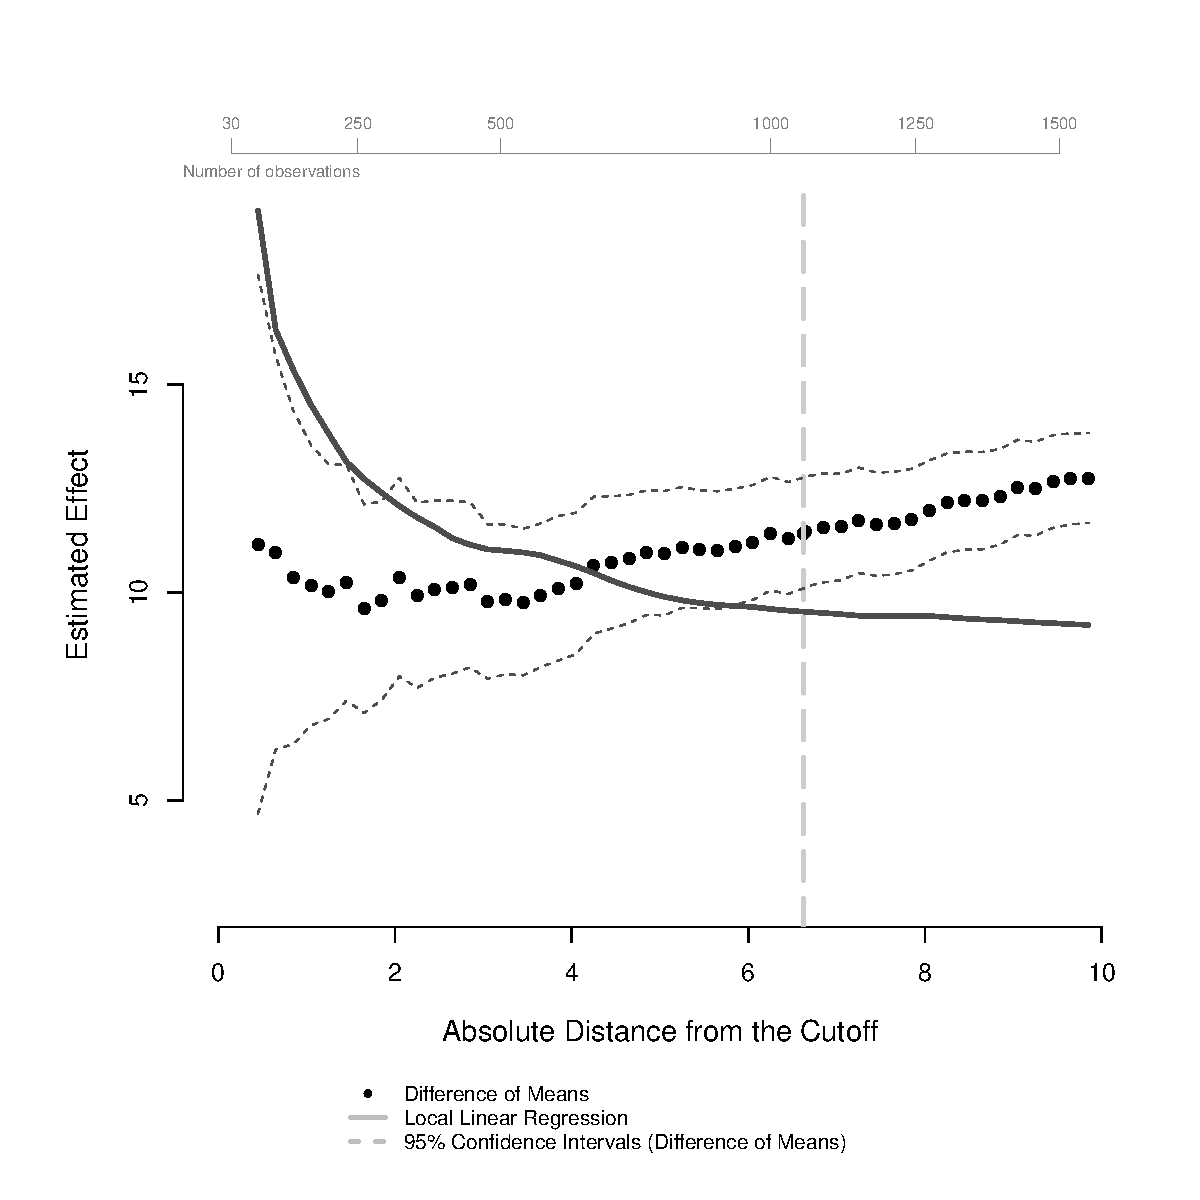
\includegraphics[width=1\textwidth]{with_add_est_plot.pdf}}
  \floatfoot{Note: Dashed gray line at the optimal bandwidth estimated by the method of \citet{imbens2011optimal}. Difference of means is the average difference in vote share for an incumbent party minus the average vote share for a non-incumbent party. The local linear regression regression uses a triangular kernel.}
  \end{figure}
\clearpage

Figure 2 follows the same logic described for Figure 1 but reports balance tests: each plot shows the effects of incumbency on a pre-treatment covariate as a function of the running variable.\footnote{In these plots, we chose to omit the axis with the number of observations because even though there are different rates of missing observations for covariates, the number of observations for the windows we were mostly interested in did not vary substantially from those in Figure 1.} These plots allow for an extensive examination of the sensitivity of balance to different windows, reporting the magnitude of the difference between treatment and control and its confidence interval. For a given identifying assumption (such as continuity of potential outcomes or as-if random assignment near the threshold), Figures 1 and 2  help the reader to evaluate whether or not -- or for which window -- these assumptions are plausible.

For instance, panel (a) in Figure 2, reports the difference in previous Democratic victories between the incumbent and non-incumbent party and shows a large imbalance, strikingly larger for smaller windows -- a point made by \citet{caughey2011elections}. Panel (b) in Figure 2 shows the difference in voter turnout between treatment and control districts. For the entire set of windows covered by the plot the difference is never statistically different from zero, suggesting that the groups are balanced in terms of this covariate. Note that the size of the difference between treatment and control is much smaller in panel (b) than in panel (a) -- also, relatively to the size of the effect of incumbency, the imbalance in panel (a) is substantial.\footnote{See Figure A.2 in the online Appendix for a the standardized effect of incumbency on vote share.}

For ease of presentation, here we present plots for only two pre-treatment covariates. However, analysts should be encouraged to present plots for all pre-treatment covariates at their disposal.\footnote{An extensive set of balance plots for pre-treatment covariates in \citet{caughey2011elections} can be found in Figure A.3 of the online Appendix.} Some plots may be more informative than others, for instance, because some pre-treatment covariates are expected to have a stronger prognostic relationship to the outcome. However, presentation of balance plots for the full set of available pre-treatment covariates may reduce opportunities for intentional or unintentional fishing.

\clearpage
\begin{figure}
\vspace{5mm}
\caption{Tests for balance: Standardized difference of means of pre-treatment covariates by Democratic margin of victory (95\% confidence intervals), U.S.\ House of Representatives, from 1942 to 2008.}\label{fig:balancepartial}
    \centering
    \begin{subfigure}{.50\linewidth}
        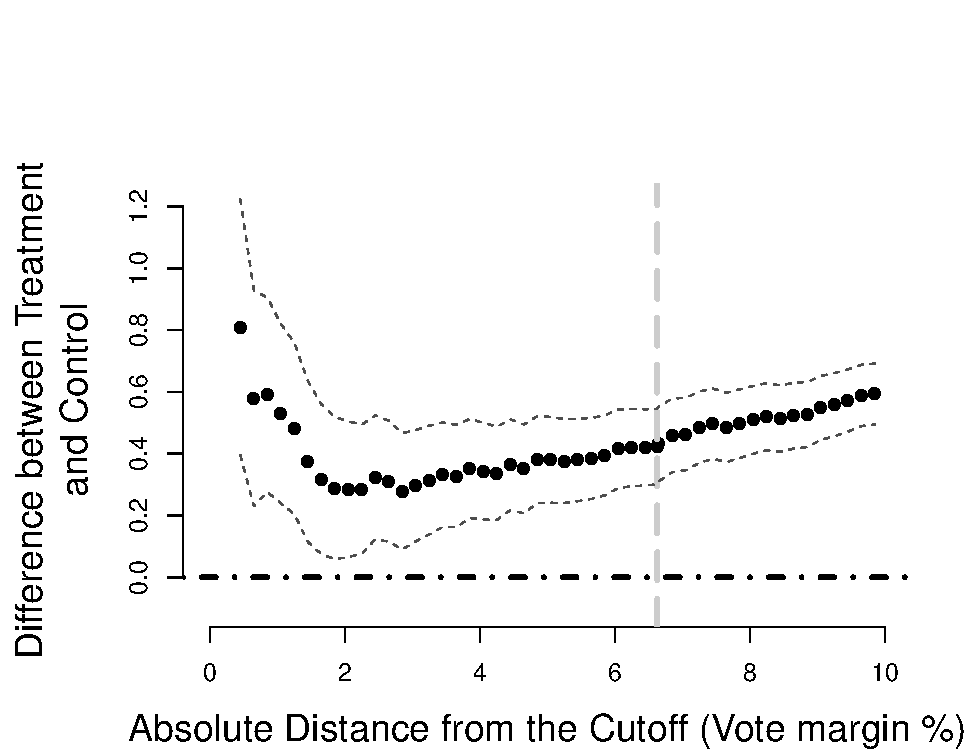
\includegraphics[scale=0.5]{balance_plot_1.pdf}
        \caption{Democratic Win in t - 1}
    \end{subfigure}
    \hskip1em
     \begin{subfigure}{.40\linewidth}
        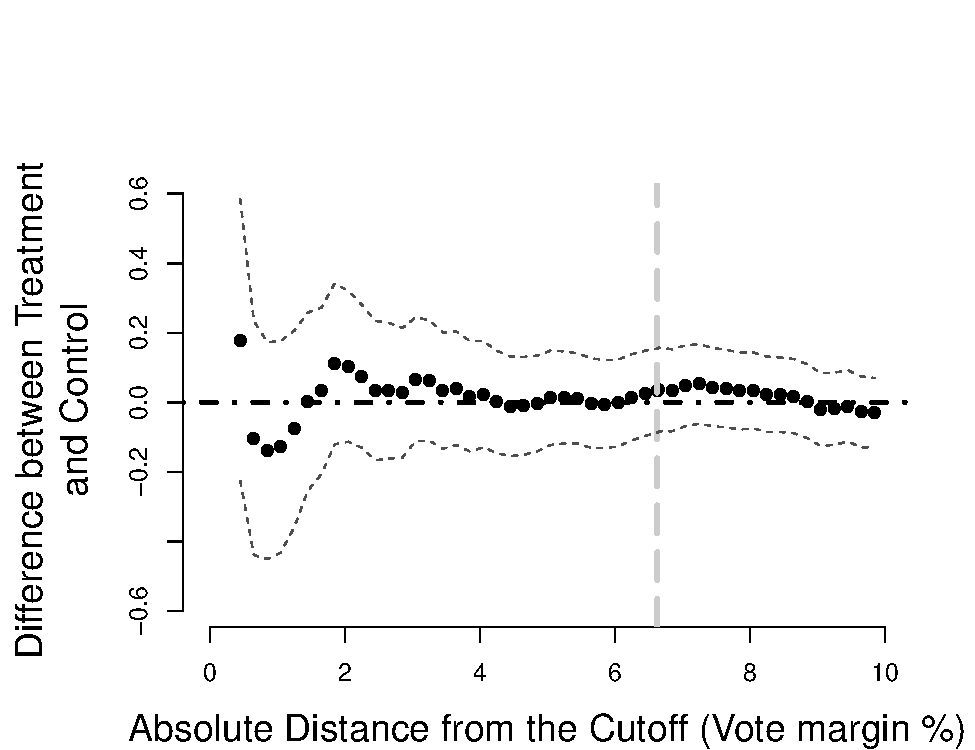
\includegraphics[scale=0.5]{balance_plot_2.pdf}
        \caption{Voter Turnout \%}
    \end{subfigure}
    \floatfoot{Note: Dashed gray line at the optimal bandwidth estimated by the method of \citet{imbens2011optimal}. Difference of means is the average difference in vote share for an incumbent party minus the average vote share for a non-incumbent party.}
    \end{figure}
\clearpage


\section*{Concluding Remarks}

We believe that these simple plots are a useful complement to the standard way in which scholars report results and balance tests from regression-discontinuity designs. They provide a simple visual comparison of how different estimators perform as a function of different windows, communicating the robustness of the results. Moreover, using these plots both for analysis of effects and placebo tests enables an informal visual inspection of how important confounders may be, relative to the size of the effect -- this is particularly informative when researchers use pre-treatment values of the outcome variable as a placebo test. However, researchers may also compare the size of treatment effects relative to other placebo tests by using standardized effect sizes across different windows, so that the scale of all plots is comparable. In summary, these plots improve the communication of findings from regression-discontinuity designs by showing readers the results from an extensive set of bandwidths, thus reducing researchers' latitude in presentation of their main findings and increasing the transparency of RD design applications.




% \theendnotes

\clearpage
\bibliographystyle{apsr}	
\bibliography{RDnote}


\end{document}
